\documentclass[12pt,titlepage]{article}
\usepackage[ngerman]{babel}
\usepackage[utf8]{inputenc}
\usepackage[]{inputenc}
\usepackage[T1]{fontenc}
\usepackage{color}
\usepackage[a4paper,lmargin={2cm},rmargin={2cm},
tmargin={2.5cm},bmargin = {2.5cm}]{geometry}
\usepackage{amssymb}
\usepackage{amsthm}
\usepackage{amsmath}
\usepackage{graphicx}
 \usepackage{listings}
 \usepackage{tocloft}
\usepackage{kpfonts}
\usepackage[explicit]{titlesec}
 \lstset{
  literate= {Ö}{{\"O}}1 {Ä}{{\"A}}1 {Ü}{{\"U}}1 {ß}{{\ss}}2 {ü}{{\"u}}1
 {ä}{{\"a}}1 {ö}{{\"o}}1
 }
\usepackage{graphicx}



\begin{document}
\begin{titlepage}
\title {Projektdokumentation Angular JS 2 \newline show4you | Eventapp}
\date{12.07.2016}
\author{Jorge Ayala und Jörg Kandzioraaaaaaaaaaaa}
\maketitle
\end{titlepage}
\newpage

\tableofcontents

asdfa 
\newpage

\part{Idee und Ziel}
\section{Idee}
Jörg hatte die Idee eine Anwendung mit Angular2 zu erstellen, bei der man Events eintragen und verwalten kann. Zusätzliche soll diese Anwendung Zwei API's von Google verbunden sein. Man soll mit Google Maps sehen wo diese Events stattfinden und man soll das Datum und die Uhrzeit direkt in seinen persöhnlichen Google Calendar eintragen können. In der eigentlichen Anwendung gibt es ein Formular, bei dem man alle wichtigen Daten zur Veranstaltung eintragen kann. Es gibt eine Liste die alle Events anzeigt und wenn man auf ein einzelnes Event klickt bekommt man die details.

\section{Ziel Definition}
Wir haben uns zum Ziel gesetzt diverse Angular2 Funktionen und Attribute dafür zu verwenden. Zum einen Nuten wir Datenobjekte(Models) mit denen wir Venue, Datum/Uhrzeit, Bands, Genre etc darstellen. Mit einer Listenansicht sollen die verschiedenen Events angezeigt werden. Mit der Einbindung der Google Maps Api soll dann noch angezeigt werden wo sich die Venues befinden. In den Event Details, die Angezeigt werden wenn man auf ein einzelnes Event klickt, soll man das Event seinem persönlichen Google Calendar hinzufügen können. Mittels Routing erstellen wir unterseiten, wie maps(hier werden alle aktuellen Veranstaltungen angezeigt), calendar(hier soll der persönliche google calendar eingeblendet werden(Monatsansicht)), Add shows(hier soll man neue Veranstaltungen hinzufügen können).


\newpage
\part{Erstellung einer einfachen Angular2 App}
\section{Erste Editierung}
Zum Anfang hat Jörg eine App mit Hilfe des Tutorials "Tour Of Heroes" erstellt. Hier wurde erstmal die Grundstruktur erstellt und mit app.component.ts die erst ts Datei. In der app.component.ts wurde dann unsere erste Klasse AppComponent erstellt von der alles aus gehen soll. Zudem haben wir die Klasse Show erstellt, welche als Atribute erstmal nur eine id und einen Namen bekommen haben. Beispielsweise wurde auch gleich eine Show erstellt. Eine Template wurde erstellt, welches die erste Ausgabe darstellt und direkt unsere erste Show anzeigt. Mit {{show.name}} und {{show.id}} könnnen wir uns die Show ausgeben lassen. Mit <input> und [(ngModel)] gehen wir dann zum two way binding und können unsere Show in Echtzeit verändern. Somit steht unsere erste kleine Anwendung. Die Html Tags die für die Ansicht da sind werden im @Component, welches mit {Component} from '@angular/core'; importiert wird, mit template eingefügt.  Hier ist auch der selector definiert bei dem man den App namen angibt.

\section{Interaktion und Detail Ansicht + Styling}
Jörg hat dann an der Liste gearbeitet die die Shows anzeigen soll und die Detailansicht, welche die Details der einzelnen Shows anzeigen soll. Zudem stylen wir die Liste. Als ersten haben wir mit cont SHOWS: Show[] = [{ .... }] einen Array von einigen Shows erstellt. Mit public shows = SHOW machen wir die property dann öffentlich. Mi *ngFor="let show of Shows" lassen wir uns dann alle shows aus dem eben erstellten array auflisten. 

\subsection{Detail Ansicht mit +ngif}
Jorge hat dann in die liste mit (click)="onSelect(show)" die einzelnen Events auswählbar gemacht. Mit *ngIf="selectedShow" konnte das event binding an eine neue Ansicht gebunden werden. Mit {{selecteShow.id}} wurde somit erstmal die Id der einzelnen Show mittels rauf klicken angezeigt. Das Problem ist, dass das jetzt noch alles recht unschön in einer Datei drinnen ist.

\newpage
\part{Components, Services, Html Auslagerung Jörg || Parrallel neue Angular2 update und Http Jorge}
\section{Components}
Jörg hat dann mittels components die einzelnen Abschintte ausgelagert.Statt mit template kann man mit templateUrl: '' die die html Tags auslagern in einer extra html Datai.  Mit styleUrls: [''] kann man dann auch noch das Styling auslagern. Und schon sieht die Datei gleich übersichtlicher aus. Jetzt wird eine richtig Componente erstellt. Die show-detail.component.ts soll nur für die Details der Shows da sein. Und die show.ts nur für eine einzelne schow, also die Definition der einzelnen Attribute(bis jeztzt nur Name und Id). In unserer app.component.ts können wir die beiden Components dann importieren. Sobald die importiert sind können wir alles aus den Compents jetzt zum Beispielt in unserer ausgelagerten Html Datei benutzen.

\begin{figure}[h]
\begin{center}
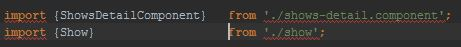
\includegraphics[scale=1.2]{links/import_erste_components.jpg}
\label{scene_intro_scale}
\end{center}
\end{figure}

\subsection{show.ts}
In die shot.ts kommt erstmal nur die Klasse Show rein, in der wie die id und den namen mit number und string definieren. Die KLasse muss natürlich mit "export class Show" exportiert werden, damit wir sie woanders benutzen können. 

\subsection{show-detail.component.ts}
Die Component ist dann schon aufwendiger. Hier wird erstmal auch die shot.ts importiert wie in der app.component.ts. Zudem brauchen wir hier auch das Component und wollen das <Input feld ja verwendne also muss man das mit import { Component, Input } from '@angular/core'; auch einbinden. Im @Component ({}) wird dann auch ein template eingebunden welches wir auch mit templateUrl auslagern können, da hier aber auch in Zukunft nicht mehr viel hinzu kommt wird es direkt in die Datei geschrieben. Wir erstellen dann noch die Klasse ShowDetailComponent die wie oben exportiert wird. Hinein kommt @Input() show: Show; die wir ja dann anzeigen lassen wollen.


\newpage
\section{Services}
Jetzt erstellen wir für unser Projekt einige services. Dazu erstelle ich erstmal eine mock-show.ts welche nur dafür dient die Attribute unserer show zu haben. Sie importiert von show.ts und exportiert selber mit SHOWS: Show []= [...] eine Liste von Shows mit deren Attributen. Hier füge ich gleich mal unseren weiteren Attribute hinzu. Dann kommt die show.service.ts welche Show von der hero.ts und SHOWS von der mock-show.ts importiert. Zudem wird injectable von @angular/core importiert. Mit @injectable() können wir die Klasse ShowService exportieren, welche eine getter Methode hat. Mit return Promis.resolve(Shows). In der app.component.ts wird ShowService importiert und in der @Component beim neuen Feld providers: mit [ShowService] hinzu gefügt. Zusätzlich brauchen wir jetzt einen Constructor der private showService: ShowService deklariert. Mit folgenden Methode können wir uns dann die Shows holen.

\begin{figure}[h]
\begin{center}
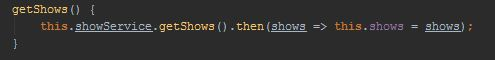
\includegraphics[scale=1.2]{links/getShows.jpg}
\label{scene_intro_scale}
\end{center}
\end{figure}

\newpage
\section{Angular2 Update}

\newpage
\section{Http}

\newpage
\section{Routing}

\newpage
\section{Maps Api}

\newpage
\section{Calendar Api}

\newpage
\section{Finalisierung}

\newpage

\section{Weiteres}
\subsection{Literatur}
\begin{itemize}
\item K. Suffer – Ray Tracing from Ground Up – Kapitel 13
\item P. Shirley – Fundamental of Computer Graphics – Kapitel 19
\end{itemize}
\subsection{Grafiken und Quellen}
Stephan Rehfeld: http://rehfeld.beuth-hochschule.de/

 
   
\end{document}